\subsection{Solar cells}

Most solar cells made are crystalline, meaning the structure of atoms is ordered, or periodic. Generally the crystals will contain imperfections and impurities. Some solar cell materials however, is not crystalline, but are missing periodicity. These solar cells are made from amorphous materials.

\subsubsection{Bandgap}

A free electron in vacuum can posses any energy. An electron in a crystal is bound by an energy gap divided by energy positions the electrons can't possess. Every available energy state can only room two electrons according to the Pauli principle. For a crystal, the energy bands can be viewed as an overlap in between single electron energy states. This can be viewed as the crystals 'electron'-shell.

\begin{figure}[H]
 \centering
 	% Tegning
 	\begin{tikzpicture}[scale=0.5]
     	\draw[very thick,->] (1,6) -- node[below] {x}  (25,6); % X akse
    	\draw[very thick,->] (1,6) -- node[left] {\begin{sideways}Energy\end{sideways}} (1,18); % Y akse
    
    \begin{scope} % Valens og ledningsb�nd
		    \draw[thick,fill=black!10] (2,7) rectangle node {Valence band} ++(22,4);
        \draw[thick,fill=black!10] (2,13) rectangle node {Conduction band} ++(22,4);
        \draw[thick,<->] (13,13) -- node[right] {Band gap} (13,11); % Pil
    \end{scope}
    \end{tikzpicture}    \caption{Energy bands}
    \label{fig:energiband}
\end{figure}

The upper band is called conduction band, and the band right below it, is called the valence band. In between these two, are the ideally forbidden band gap. This band gap is very important in relations with solar cells, and is often given in the units of electron volts (eV).

For electrons to move out of the crystal, they have to be in the conduction band. For electrons to get to the conduction band, they need to have enough energy to move from the valence band. This can happen if the electron has enough thermal energy, or receive energy from the outside, like light. This gives the material increased conductivity. In addition to this, there will be a free state in the valence band, which results in a less probability of collisions among the remaining electron, which lead to a higher mean kinetic energy of the electrons in the valence band. This also contribute to a better conductivity for the material. 

For light to excite an electron from the valence band to the conduction band, it needs to have equal, or more energy than the band gap. Energy of light in electron volts is given by:

\begin{equation}
E=h\nu =\frac{hc}{\lambda}
\label{eq:light_energy}
\end{equation}

where $E$ is energy in electron volts, $h$ is Planks constant (4.13\cdot10$^-{15}$~eV\cdot s), $\nu$ is frequency, $\lambda$ is wavelength, and $c$ is the speed of light (3\cdot10$^8$~m/s). 1~eV corresponds to 1240~nm.

Materials is often divided into three categories; Isolators, semiconductors, and conductors. Isolators have none, or few electrons in the conduction band, which gives them poor conductivity. Conductors often have filled conduction bands in room temperature, which provide good conductivity. Even at 0K, conductors have a partially filled conduction band. Semiconductors on the other hand, does not have any electrons in the conduction band at 0K. Semiconductors have lower conductivity than conductors, but better than isolators. The bandgap for semiconductors lay in between that of the conductors and isolators. At room temperature semiconductors have a partially filled conduction band.

\begin{figure}[H]
 \centering
 % Tegning
 

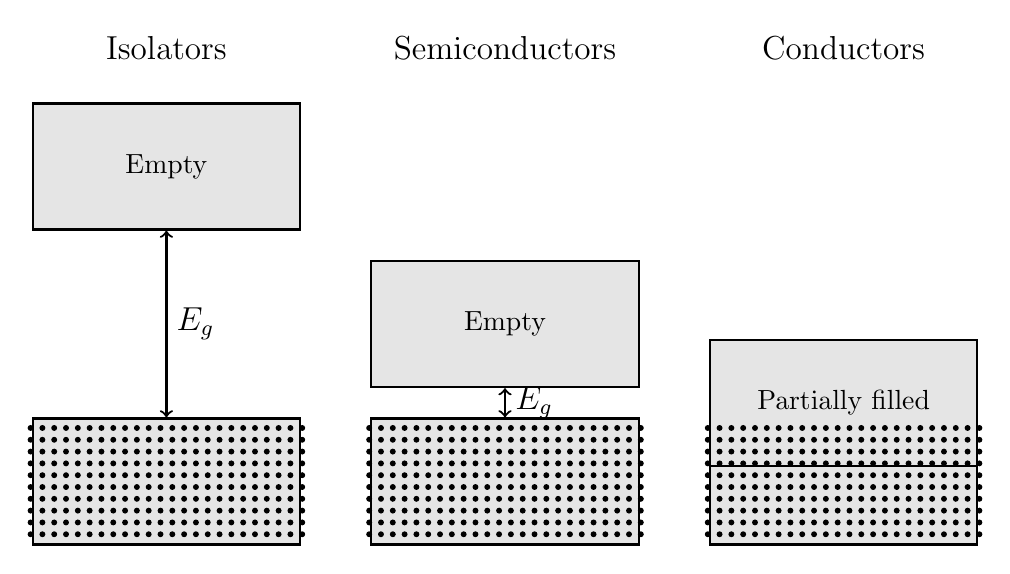
\begin{tikzpicture}
 	% Styles til elementer (kan ogs� v�re generelle utenfor tikzpicture)
	\tikzstyle{ledningsband} 	=	[rectangle, draw, thick, fill=black!10, text width=9em, text centered, minimum height=1.6cm]
	\tikzstyle{valensband}		= [rectangle, draw, thick, fill=black!10, text width=9em, text centered, minimum height=1.6cm]


	% Boksene i bunnen
	\node[valensband]	(valens_isolator)																										{};
	\node[valensband]	(valens_halvleder)	[right of=valens_isolator,  node distance=4.3cm]	{};
	\node[valensband]	(valens_metall)			[right of=valens_halvleder, node distance=4.3cm]	{};	
	
	% Boksene i toppen
	\node[ledningsband]	(lednings_isolator)		[above of=valens_isolator, 	node distance=4cm]	{Empty};
	\node[ledningsband]	(lednings_halvleder)	[above of=valens_halvleder, node distance=2cm]	{Empty};
	\node[ledningsband]	(lednings_metall)			[above of=valens_metall, 		node distance=1cm]	{Partially filled};
	
	% Piler
	\draw[thick,<->] (valens_isolator)  -- node[right] {\large $E_g$} (lednings_isolator);
	\draw[thick,<->] (valens_halvleder) -- node[right] {\large $E_g$} (lednings_halvleder);
	
	% Tekst p� toppen
	\node (isolator_tekst)  [above of=lednings_isolator,node distance=1.5cm]	{\large Isolators};
	\node (halvleder_tekst) [right of=isolator_tekst, 	node distance=4.3cm] 		{\large Semiconductors};
	\node (metaller_tekst)  [right of=halvleder_tekst, 	node distance=4.3cm] 		{\large Conductors};
	
	% Elektroner i valensb�nd
	\foreach \y in {0,0.15,...,1.4}
		\foreach \x in {0,0.15,...,3.5} {
			\draw (\x-1.725,\y-0.67) circle (0.03cm) [fill=black];	% Isolator
			\draw (\x+2.575,\y-0.67) circle (0.03cm) [fill=black];	% Halvleder
			\draw (\x+6.875,\y-0.67) circle (0.03cm) [fill=black];	% Metall
		}	
	
\end{tikzpicture}

	    \caption{Typical bandgaps at 0K} 
 \label{fig:bandgap}
\end{figure}
\vspace{10mm}

Typical bandgap for semiconductor silicon is E$_g$=1.1~eV, compared with 5~eV for diamond, which is an isolator \cite{streetman}.

Holes is a description of missing electrons in the valence band. A hole will appear when an electron is excited from the valence band into the conduction band. With a small bandgap, and high temperatures, there will be a considerably larger amount of electrons in the conduction band, compared to low temperatures, and a large bandgap. This is described by law of mass action

\begin{equation}
np=N_cN_ve^{-\frac{E_g}{kT}}
\label{eq:massevirkningsloven}
\end{equation}

where $n$ is number of electrons, $p$ is number of holes, $N_c$ and $N_v$ is constants for a given material, $E_g$ is the bandgap, $k$ is Boltzmanns constant (1.38\cdot10$^-{23}$~m$^2$kgs$^{-2}$K$^{-1}$), and $T$ is temperature in Kelvin. For an intrinsic semiconductor, meaning a semiconductor without any doping atoms, like a pure silicon crystal, the law of mass action can be written as

\begin{equation}
np=n_i^2
\label{eq:massevirkningsloven_intrinsikk}
\end{equation}

where

\begin{equation}
n_i=\sqrt{N_c N_v}e^{-\frac{E_g}{2kT}}
\label{eq:intrinsikk}
\end{equation}


\subsubsection{Doping}

By adding certain atoms of a different type than those constituting the semiconductor itself, it is possible in increase the concentration of electrons in the conduction band without a concomitant increase on the number of holes in the valence band. This is called donor-doping. An example of donor doping is added phosphorous into a silicon crystal. This will result in more electrons in the conduction band, due to phosphor having one more valence electron than silicon. The doping is usually so small that the band structure won't be affected. By adding phosphorous this way, one has increased electrons, $n$, without increasing holes, $p$. This is called donor doping. If you instead of phosphor, add boron, the material will be acceptor doped. This is due to boron having one less electron in the valence band than silicon, and would result in an extra hole in the valence band of the crystal. Usually the number of dopants in silicon are substantially larger than the intrinsic concentration, $n_i$, so that

\begin{equation}
n \approx N_d
\label{eq:donordoping}
\end{equation}

for donor doping, and

\begin{equation}
p \approx N_a
\label{eq:akseptordoping}
\end{equation}

for acceptor doping where $N_d$ is donor concentration, and $N_a$ is acceptor concentration.

A doped semiconductor is generally called extrinsic \cite{streetman}. If a semiconductor is doped with a number of donor atoms, it is called n-doped or n-type, due to there being more electrons than holes. For acceptor doping, it is called p-doped, or p-type, semiconductor. The dominating charge carrier in the semiconductor are called majority carriers. The other charge carrier, i.e. holes in the n-type semiconductor are called minority carriers.

\subsubsection{Transport and recombination processes}

There are two mechanisms that contribute to transport of electrons and holes in semiconductors: drift, and diffusion. Drift is a transport of a charge carrier due to an electric field. For transport of a hole in one dimension, the current $I_p$ is equal to the amount of holes $N_p$ times the charge $q$ crossing a cross-sectional area.

\begin{equation}
I_p = N_p q
\label{eq:drift}
\end{equation}

In vacuum, an electric field would accelerate the electrons, and the velocity would increase indefinitely. In solids, however, interactions of collisions with other species in the solid leads to a resistance towards the drift of the charged particles, and after an initial acceleration the mean velocity becomes constant in a constant electric field. This average drive velocity, denoted $v_p$ for holes, is related to the electric field $E$ through the hole mobility $�_p$

\begin{equation}
v_p = �_p E
\label{eq:electronspeed}
\end{equation}

If all the electrons is moving in the same direction, the current per area is given by

\begin{equation}
J_p = \frac{I_p}{A} = \frac{N_p q}{A} = pAv_p \frac{q}{A} = pv_p q = pq�_p E
\label{eq:hulltetthet}
\end{equation}

combined with a similar expression for electrons

\begin{equation}
J = J_p + J_n = (nq�_n + pq�_p)E = \sigma E
\label{eq:stromtetthet}
\end{equation}

where $�_n$ is the mobility for electrons, $\sigma$ is the semiconductors conductivity, and $J_n$ is the current density due to the concerted movement of electrons. It is also usual to define the resistivity of the semiconductor as the inverse of its conductivity. The current is then obtained by

\begin{equation}
I = JA = A\sigma E = \left( \frac{A\sigma}{L}\right)V = \frac{V}{R}
\label{eq:current}
\end{equation}

which is recognized as Ohm's law.


Diffusion is a transport process caused by the random motion of the diffusing particles in the medium in which they diffuse. The net transport of particles is in the opposite direction of the concentration gradient. For holes we have

\begin{equation}
N_p=-D_p\frac{dp}{dx}
\label{eq:diffusion}
\end{equation}

where the proportionality constant $D_p$ is the diffusion coefficient (m$^2$/s) for holes.

The movement of charged particles are frequently determined by the simultaneous presence of electric fields and concentration gradients. Both of the relevant transport parameters, mobilities and diffusion coefficients, will in general depend on temperature. The relation between diffusion coefficient and mobility is

\begin{equation}
\frac{D_p}{�_p}=\frac{kT}{q}
\label{eq:transport_relation}
\end{equation}

for holes, and a corresponding one exist for electrons.

\subsubsection{Excitation and recombination}

Electrons can move from one band to another directly, or indirectly. In indirect generation and recombination the electrons can employ the so-called gap-states. Such conditions will always exist in semiconductors and are related to impurities, defects in the crystal structure, boundary surfaces (grain boundaries) and surfaces. Gap-states are in between the valence band and the conduction band, which is not allowed states in a perfect crystal.


\begin{figure}[H]
\centering
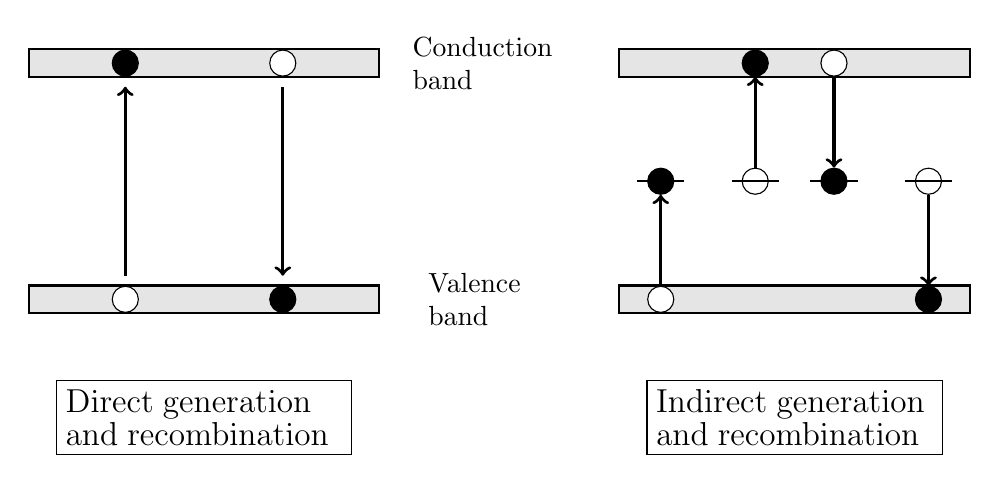
\begin{tikzpicture}

% Styles til elementer
\tikzstyle{band} 	=	[rectangle, draw, thick, text width=12em, fill=black!10, text centered, minimum height=1em]
\tikzstyle{e} 	=	[circle, draw, fill=black] % radius=0.2cm
\tikzstyle{h} 	=	[circle, draw, fill=white] % radius=0.2cm

	% Direkte
	\node[band]	(direkte_valens)																									{};
	\node[band]	(direkte_lednings)	[above of=direkte_valens, node distance=3cm]	{};
	\node[e] (elektron1) [right of=direkte_valens] {}; % Elektron
	\node[h] (hull1) [left of=direkte_valens] {}; % Hull
	\node[e] (elektron2) [left of=direkte_lednings] {}; % Elektron
	\node[h] (hull2) [right of=direkte_lednings] {}; % Hull
	\draw[very thick,->] (-1,0.3) -- (-1,2.7) {} ; % Pil opp
	\draw[very thick,<-] (1,0.3) -- (1,2.7) {} ; % Pil ned
	\node (direkte_tekst) [rectangle, draw, text width=10em, below of=direkte_valens,node distance=1.5cm]	{\large Direct generation and recombination};
	
	\node (lednings_tekst) [right of=direkte_lednings, node distance=3cm, text width=2em] {Conduction band};
	\node (valens_tekst) [right of=direkte_valens, node distance=3.2cm, text width=2em] {Valence band};
	
	% Indirekte
	\node[band]	(indirekte_valens)		[right of=direkte_valens,  node distance=7.5cm]	{};
	\node[band]	(indirekte_lednings)	[above of=indirekte_valens, node distance=3cm]	{};
	
	\node[h] (h3) [left of=indirekte_valens, node distance=1.7cm] {}; % Hull
	\node[e] (e3) [above of=h3, node distance=1.5cm] {}; % Elektron
	\draw[very thick,->] (h3) -- (e3) {}; %Pil
	\draw[thick,-] (5.5,1.5) -- (6.1,1.5) {}; % Linje gjennom
	
	\node[e] (e4) [left of=indirekte_lednings, node distance=0.5cm] {}; % Elektron
	\node[h] (h4) [below of=e4, node distance=1.5cm] {}; % Hull	
	\draw[very thick,->] (h4) -- (e4) {}; % Pil
	\draw[thick,-] (6.7,1.5) -- (7.3,1.5) {}; % Linje gjennom
	
	\node[h] (h5) [right of=indirekte_lednings, node distance=0.5cm] {}; % Hull
	\node[e] (e5) [below of=h5, node distance=1.5cm] {}; % Elektron
	\draw[very thick,->] (h5) -- (e5) {}; % Pil
	\draw[thick,-] (7.7,1.5) -- (8.3,1.5) {}; % Linje gjennom
	
	\node[e] (e6) [right of=indirekte_valens, node distance=1.7cm] {}; % Elektron
	\node[h] (h6) [above of=e6, node distance=1.5cm] {}; % Hull	
	\draw[very thick,->] (h6) -- (e6) {}; %Pil
	\draw[thick,-] (8.9,1.5) -- (9.5,1.5) {}; % Linje gjennom
	
	\node (indirekte_tekst) [rectangle, draw, text width=10em, below of=indirekte_valens,node distance=1.5cm]	{\large Indirect generation and recombination};
	
\end{tikzpicture}	

\caption{Generation and recombination}%
\label{fig:indirect}%
\end{figure}

In semiconductors with direct bandgap, like GaAs, both processes will occur. In semiconductors with with indirect bandgap, like silicon, a direct process cannot happend without contributions from lattice vibrations (phonons), something which makes the process less probable. This is one of the reasons why impurities in silicon solar cells is an important parameter. The electron in an indirect process is moving in the form of a plane wave with propagation constant $\vec{k}$, also called wave vector. 


% Indirekte b�ndbap figur
\begin{figure}[H]
\centering
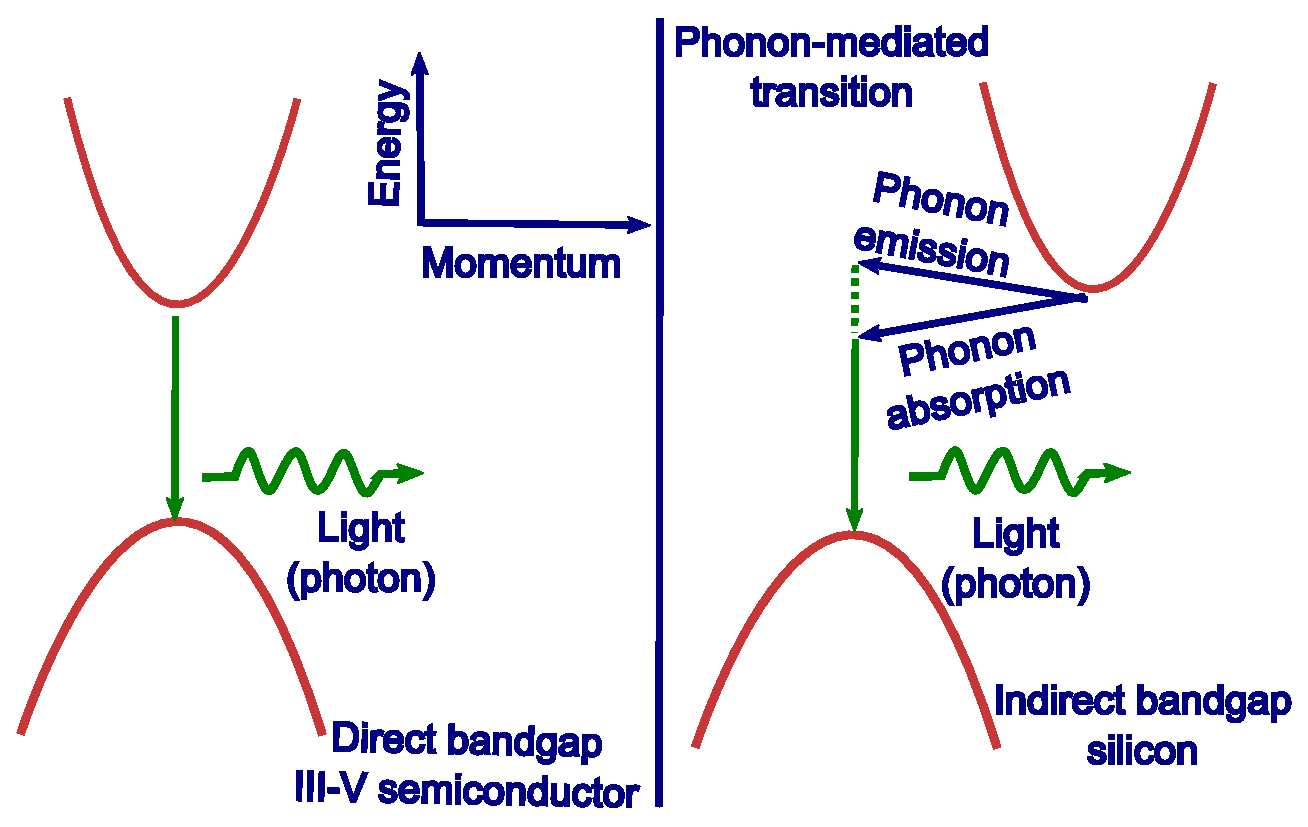
\includegraphics[width=\columnwidth]{bandgap}%
\caption{Direct and indirect recombination (figure from \cite{aps})}%
\label{fig:indirect_direct}%
\end{figure}


Generation and recombination processes can be described as net flow of electrons to the conduction band, $U_n$, proportional to the deviation from equilibrium

\begin{equation}
U_n = - \frac{n-n^0}{\tau_n}
\label{eq:generation_n}
\end{equation}

where $\tau_n$ is the lifetime of electrons, which is the time that an electron in the conduction band traveling at mean speeds, in the conduction band use before recombining with a hole. $n$ is the concentration of electrons and $n^0$ is the equilibrium concentration of electrons, $n^0=n_i^2$. Similarly, the net production of holes $U_p$

\begin{equation}
U_p = - \frac{p-p^0}{\tau_p}
\label{eq:generation_p}
\end{equation}

\subsubsection{Solar cell}

In a semiconductor with one p-doped, and one n-doped area laying next to each others is called a pn-junction. A pn-junction has rectifying properties, meaning the electrical conductance are significantly better in one direction than the other, in contrast to a resistor for which it does not matter, as the voltage drops across the resistance whether the current runs one way or another through it. This rectifying behavior defines a diode. Due to the p-side having a larger concentration of electrons in the conduction band than the n-side, there will be a net transport of conduction band electrons from the n-side, to the p-side by diffusion. The same is also happening for holes from the p-side to the n-side. This net flow of charge is called the diffusion current. In principle, the dopants of Si, B, and P can also diffuse between the two parts of the crystal. Such a transport will only be significant at the temperature range of 800 to 900$^\circ$~C, and can be neglected at  temperatures like room temperature.

% figur fra s. 14 i kompendiet

\begin{figure}[H]%
\centering
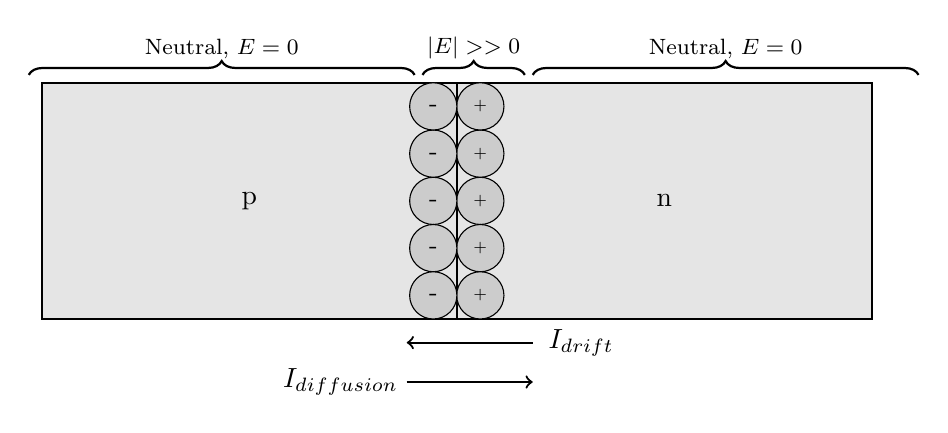
\begin{tikzpicture}

	\tikzstyle{box} 	=	[rectangle, draw, thick, fill=black!10, minimum width=15em, minimum height=3cm]
	\tikzstyle{ladning} 	=	[circle, draw, fill=black!20, minimum size=0.6cm]
	\def\edistance{0.6cm}
	
	\node[box]	(p)	{p};
	\node[box]	(n) [right of=p, node distance=15em]	{n};
	
	\node[ladning] (p3) [right of=p, node distance=8.35em] 	{\tiny{+}};
	\node[ladning] (p2) [above of=p3, node distance=\edistance] {\tiny{+}};
	\node[ladning] (p1) [above of=p2, node distance=\edistance] {\tiny{+}};
	\node[ladning] (p4) [below of=p3, node distance=\edistance] {\tiny{+}};
	\node[ladning] (p5) [below of=p4, node distance=\edistance] {\tiny{+}};
	
	\node[ladning] (n3) [left of=n, node distance=8.35em] 			{\small{-}};
	\node[ladning] (n2) [above of=n3, node distance=\edistance] {\small{-}};
	\node[ladning] (n1) [above of=n2, node distance=\edistance] {\small{-}};
	\node[ladning] (n4) [below of=n3, node distance=\edistance] {\small{-}};
	\node[ladning] (n5) [below of=n4, node distance=\edistance] {\small{-}};
	
	% Draw curly braces using path decoration
	\draw [thick,decorate,decoration={brace,amplitude=5pt}]
   (2.2,1.6) -- (3.5,1.6)
   node [black,midway,above=2pt] {\footnotesize $|E|>>0$};

	\draw [thick,decorate,decoration={brace,amplitude=5pt}]
   (-2.8,1.6) -- (2.1,1.6)
   node [black,midway,above=2pt] {\footnotesize Neutral, $E=0$};

	\draw [thick,decorate,decoration={brace,amplitude=5pt}]
   (3.6,1.6) -- (8.5,1.6)
   node [black,midway,above=2pt] {\footnotesize Neutral, $E=0$};

	% Str�mpiler
	\draw [thick,<-] (2,-1.8) -- (3.6,-1.8) node [right=2pt]	{$I_{drift}$}; 
	\draw [thick,->] (2,-2.3) -- (3.6,-2.3) node [left=45pt]	{$I_{diffusion}$}; 

\end{tikzpicture}

\caption{Depletion area}%
\label{fig:depletionarea}%
\end{figure}

Each hole that leaves the p-side will leave behind an acceptor that is no longer neutralized by a hole. Similarly, each electron in the n-side leave behind a donor that is not neutralized by an electron. A layer near the interface between the two materials with non-neutral donors on the n-side and non-neutral acceptor in the p-side will form. This layer is often called the depletion layer, since it is essentially depleted of free charge carriers. Since the n-side of the depletion layer contains non-neutral donors this side will be positively charged. The corresponding p.side will be negatively charged. These charges therefore will cause an electric field directed from n-to p-side, or a corresponding drop in electrical potential from the n-side to the p-side. This electrical potential is resulting in a drift current which is moving in the opposite direction of the diffusion current which is resulting in equilibrium, meaning zero net flow of current.

By exposing the pn-junction to light, minority carriers may be generated beyond those generated thermally. The carriers are generated by photon absorption. This generation is usually significantly greater than the drift current. A diode not exposed to light has the following current voltage characteristic:

\begin{equation}
I=|I_{drift}|e^{\frac{qV}{kT}-1}
\label{eq:diodeiv}
\end{equation}

When the diode is exposed to light, the drift current is increased, and the current voltage characteristic is changing as seen in figure \ref{fig:ivsolcelle}.

% figur fra side 22 i kompendiet
\begin{figure}[H]
\centering
\begin{tikzpicture}

	\draw [->] (-3,0) -- (3,0) node [right=5pt]	{V};  % Y-akse
	\draw [->] (0,-2) -- (0,3) node [above=5pt]	{I}; % X-akse

	% Diode
	\draw [dashed,-] (-3,-0.2) -- (-1,-0.2);
	\draw [dashed,-] (-1,-0.2) .. controls +(right:1.2cm) .. (1.5,3);
	\draw [->, >=triangle 45] (-2.5,0.5) -- node[right] {$I_{drift}$} (-2.5,0);
	\draw [->, >=triangle 45] (-2.5,-0.7) -- (-2.5,-0.2);
	
	% Solcelle
	\draw [-] (-3,-1.8) -- (-1,-1.8);
	\draw [-] (-1,-1.8) .. controls +(right:1.5cm) .. (1.5,2);
	\draw [<->, >=triangle 45] (-1.7,-1.8) -- node[right] {$I_{light}$} (-1.7,-0.2);

\end{tikzpicture}

\caption{Current-voltage characteristics for a solar cell}%
\label{fig:ivsolcelle}%
\end{figure}

For solar cells, the current going out of the cell is usually defined as positive, so that the characteristic is flipped upside-down

\begin{equation}
I=I_{light}-I_{drift}(e^{\frac{qV}{kT}-1})
\label{eq:solarcelliv}
\end{equation}

where $I_{light}$, is the current generated by the exposing light. In an open circuit the voltage is defined as 

\begin{equation}
V_{OC}=\frac{kT}{q}\ln(\frac{I_{light}}{I_{drift}}+1)
\label{eq:voc}
\end{equation}

and max power defined as

\begin{equation}
P_m=I_m V_m
\label{eq:piv}
\end{equation}

where $P_m$ is maximum power, $I_m$ is maximum current and $V_m$ is maximum voltage. Solar cell efficiency is defined as 

\begin{equation}
\eta=\frac{P_m}{P_{inn}}=FF \frac{I_{belysning} V_{OC}}{P_{inn}}
\label{eq:virkningsgrad}
\end{equation}

where FF is the fill factor is given by

\begin{equation}
FF=\frac{I_m V_m}{I_{light} V_{OC}}
\label{eq:fillfactor}
\end{equation}


% fyllfaktor figur
\begin{figure}[H]
\centering
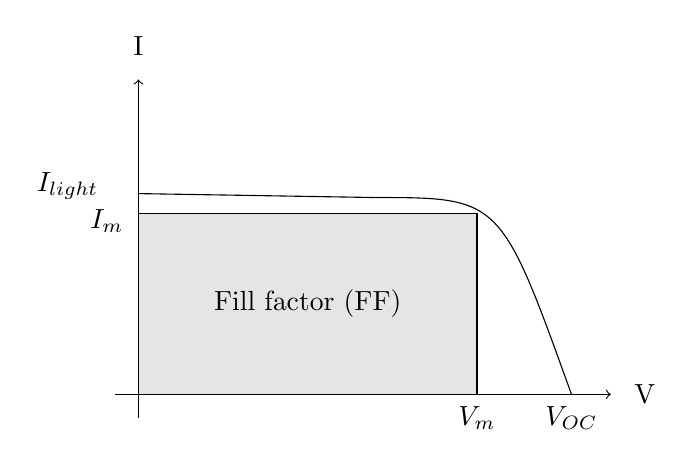
\begin{tikzpicture}

	\draw [->] (-0.3,0) -- (6,0) node [right=5pt]	{V};  % X-akse
	\draw [->] (0,-0.3) -- (0,4) node [above=5pt]	{I}; % Y-akse

	% Faktisk kurve
	\draw [-] (0,2.55) -- (3,2.5);
	\draw [-] (3,2.5) .. controls +(right:1.6cm) .. (5.5,0);
	
	% Fyllfaktor
	\node [draw, rectangle,fill=black!10,minimum height=2.3cm, minimum width=4.3cm] (FF) at (2.15,1.15) {Fill factor (FF)};
	
	% Tekst
	\node at (-0.9,2.65) {$I_{light}$};
	\node at (-0.4,2.2) {$I_m$};
	\node at (4.3,-0.3) {$V_m$};
	\node at (5.5,-0.3) {$V_{OC}$};
	
	
\end{tikzpicture}

\caption{Current-voltage characteristics with fill factor}%
\label{fig:fyllfaktor}%
\end{figure}

Solar cells with defects, have a less efficiency than clean samples

\begin{figure}[H]
\centering
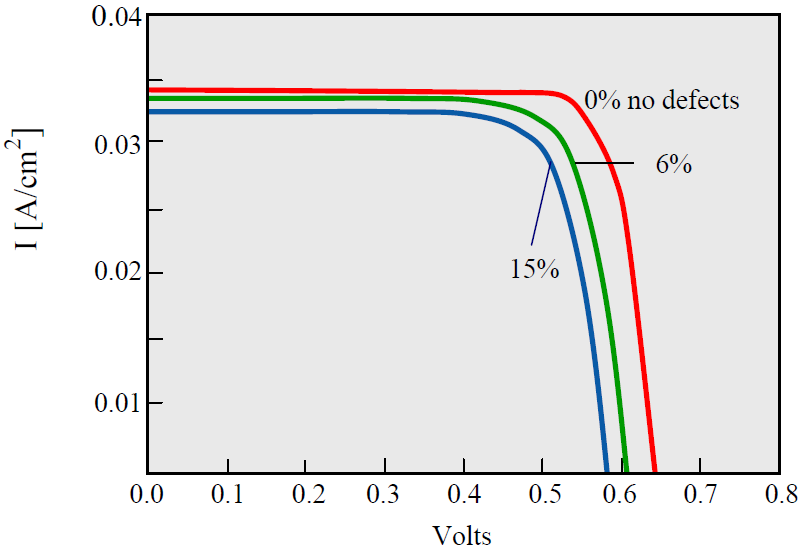
\includegraphics[width=\columnwidth]{efficiency}%
\caption[I-V characteristics with defects]{A comparison of calculated I-V characteristics of three cells with 0\%, 6\%, and 15\% of area covered by defects from \cite{sopori09}.}%
\label{fig:IVwithdefects}%
\end{figure}

which makes it important to be able to characterize defects as well as impurities in order to increase solar cell efficiency.
